\chapter{Operacionalización de Variables}
En una investigación científica, las variables son los elementos que permiten medir u observar los conceptos u fenómenos que estamos estudiando en una investigación. De manera exacta, podemos definir a una variable como cualquier característica que puede ser \textbf{medida, observar, manipular u controlar} en una experimentación u observación.

    \begin{figure}[H]
        \centering
        %\isPreprints{\centering}{} % Only used for preprints
        \caption{Tipos y características de una variable
        \label{fig-tipos-caracteristicas-variables}}    
                
        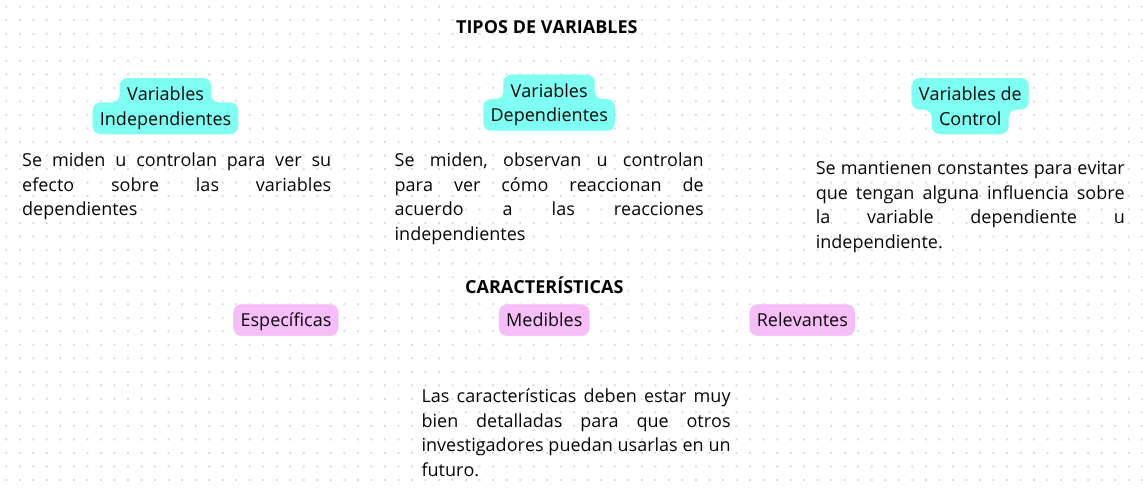
\includegraphics[width=10.0 cm]{src/imgs/tipos-variables.png}

        \vspace{0.1cm}
        % \small EN CASO DE SER BAJO ELABORACIÓN PROPIA, NO HACE FALTA AGREGAR LA NOTA
    \end{figure}

    \begin{figure}[H]
        \centering
        %\isPreprints{\centering}{} % Only used for preprints
        \caption{Ejemplo 1 - de Operacionalización de variables
        \label{fig-relacion-inversa-hipótesis}}    
                
        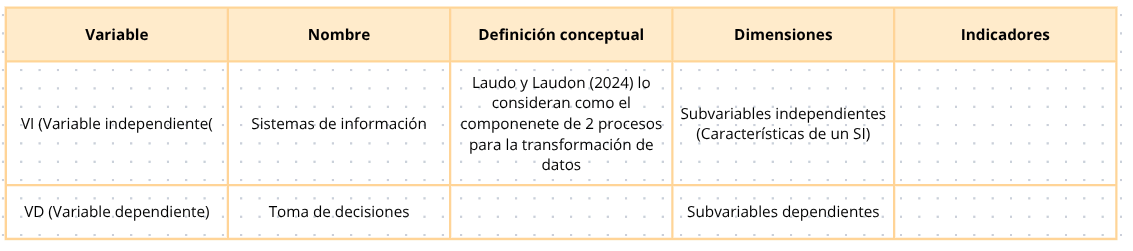
\includegraphics[width=10.0 cm]{src/imgs/operacionalizacion-variables-1.png}

        \vspace{0.1cm}
        % \small EN CASO DE SER BAJO ELABORACIÓN PROPIA, NO HACE FALTA AGREGAR LA NOTA
    \end{figure}

        \begin{figure}[H]
        \centering
        %\isPreprints{\centering}{} % Only used for preprints
        \caption{Ejemplo 2 - de Operacionalización de variables
        \label{fig-relacion-inversa-hipótesis}}    
                
        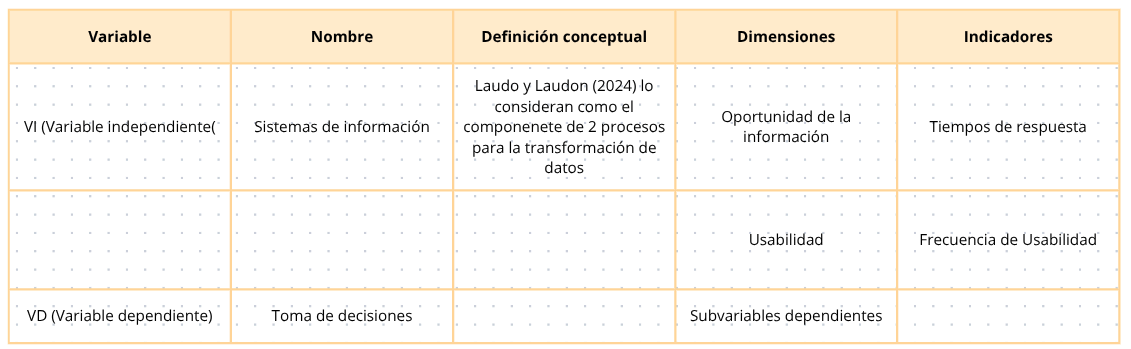
\includegraphics[width=10.0 cm]{src/imgs/operacionalizacion-variables-2.png}

        \vspace{0.1cm}
        % \small EN CASO DE SER BAJO ELABORACIÓN PROPIA, NO HACE FALTA AGREGAR LA NOTA
    \end{figure}

La definición conceptual a preferencia debe venir de teóricos (en lugar de solo autores de investigaciones).
Las dimensiones e indicadores debe salir de la teoría (De allí saldrá todo, puedes encontrarlo en otros lugares, pero a preferencia). En algunos casos también se utiliza la definición operacional. Esto será su valor matemático o algo así.

Ejemplo:
\begin{itemize}
    \item \textbf{Rentabilidad:}
    \begin{itemize}
        \item \textbf{De manera conceptual:} Es la utilidad u gannacia que tiene una empresa respecto a sus operaciones
        \item \textbf{De manera operacional:} Es la diferencia entre los ingresos  y egresos (gastos), siendo su fórmula: I - E
    \end{itemize}
\end{itemize}
